\chapter{Method}
\label{chap:method}

The Serpent 2 Monte Carlo code uses a combination of  ray tracing and
delta-tracking to simulate the propagation of particles. The \gls{wdt}
method modifies delta-tracking for an absorbing medium, replacing virtual
collisions with a weight reduction. In this chapter, we will discuss
the \gls{wdt} routine for absorption events, and extend the method to
include scattering. We will then define the \gls{wdt} threshold, a key
parameter for its implementation in Serpent 2.

\section{\Acrlong{wdt}}
\label{sec:wdt}

Morgan and Kotlyar~\cite{morgan2015} introduced a method to improve the
inefficiencies of Woodcock delta-tracking in the presence of large
absorbers. The method, \gls{wdt}, replaces the
rejection sampling algorithm of delta-tracking with a weight reduction
algorithm. This process is similar to survival biasing, or implicit capture.

\subsection{Implicit Statistical Events}
\label{sec:implicit}

We consider a process that can result in multiple outcomes, each with
their own probability. One approach is to sample a random variable and
determine which outcome actually occurred. If the event occurs many
times, we can instead replace the
statistical process by using the expected value of the random process
\cite{lux1991}. The expected value of a random variable $x$ that can
take values ${x_1 \ldots x_n}$ with  probabilities ${p_1 \ldots p_n}$, respectively,
is given by:
\begin{equation}
  \label{eq:expval}
  E[x] = x_1p_1 + x_2p_2 \ldots + x_{n}p_n
\end{equation}
For example, imagine we have a bag with four coins, three worth \$0.25 and
one worth \$0.10. The values and their probabilities are:
\begin{align*}
  x_1 = 0.25, \quad p_1 = \frac{3}{4} = 0.75 \\
  x_2 = 0.10, \quad p_2 = \frac{1}{4} = 0.25
\end{align*}
For a given draw, we could sample a random value and use the
probabilities $p_1$ and $p_2$ to determine the coin drawn. Or, we can
describe the expected value of the drawn coin:
\begin{align*}
  E[x] &= x_1p_1 + x_2p_2 \\
  &= (0.25 \times 0.75) + (0.10 \times 0.25) \\
  &= 0.2125
\end{align*}
\begin{minipage}{1.0\linewidth}
  This value represents the average value of a coin drawn, if we
  perform many draws. The following Matlab code replicates this
  procedure:
\begin{lstlisting}
v = 0;
n = 1000;
for i = 1:n
    xi = rand;  
    v = v + (xi < 0.25)*0.1 + (xi >= 0.25)*0.25;
end
\end{lstlisting}
\end{minipage}

Although the exact values will vary due to the small sample size, \verb|v/n|
$\approx 0.2125$, as we expected.

This framework is often applied to neutron propagation in a process
called ``survival biasing.'' At each collision location, the type of
interaction is sampled and the appropriate action taken. In the case
of an capture event the neutron is ``killed,'' removed from the
simulation. While this accurately reflects the physical reality, it
does not produce good statistics. Assuming we are using a collision
estimator, the neutron's contribution to our simulation is the history
of collisions. Each of these provide a score to that particular
collision, contributing to the overall simulation
statistics. Capture events that kill neutrons, therefore, are
removing the very particles we need to generate better statistics,
resulting in the need for many more particles. Mitigating this issue
is the goal of survival biasing.

Survival biasing avoids killing neutrons by replacing capture
events with an expected outcome. As described above, we do not need to
track the outcome of every single event, but can rely on the expected
value. This will give us, on average, the outcome of our many
events. To eliminate our explicit consideration of capture events,
we therefore have two possible event types: capture events, and
scattering events. The probabilities $p$ will be given by the
ratios of the cross-sections:
\begin{align*}
  p_{\mathrm{capture}} = \frac{\Sigma_{c}}{\Sigma_t} \\
  p_{\mathrm{scattering}} = \frac{\Sigma_{s}}{\Sigma_t}
\end{align*}
Where $\Sigma_{c}$ and $\Sigma_{s}$ are the macroscopic cross-sections
for capture and scattering, respectively.

In the coin example, each had a different monetary value, giving us an
expected value when we drew many times. We must introduce something
similar for neutrons. It is convention to call this intrinsic value
``weight'' and represents the importance of the neutron. All neutrons
are born with the same weight, usually unity, and are killed when they
have zero weight. By that convention a capture event that kills a
neutron immediately forces the final weight of the neutron to zero,
$w_{f,\mathrm{capture}} = 0$. We can then calculate the expected
value of the interaction of a neutron with initial weight $w_i$:
\begin{align*}
  E[w_f] &= w_{f,\mathrm{scattering}}p_\mathrm{scattering} +
           w_{f,\mathrm{capture}}p_\mathrm{capture} \\
  &= w_{f,\mathrm{scattering}}p_\mathrm{scattering}
\end{align*}
A scattering event merely changes the location of the neutron in
energy and angle phase space, leaving its importance
unchanged. Therefore, $w_{f,\mathrm{scattering}} = w_i$:
\begin{align*}
  E[w_f] = w_ip_\mathrm{scattering} 
\end{align*}
Now every collision is considered to be a non-capture event. The
neutron continues with a lower weight, proportional to the probability
that the event was scattering. The weight lost in the collision is
scored as capture:
\begin{align*}
  S_\mathrm{capture} &= E[w_i - w_f] \\
  &= E[w_i] - E[w_f] \\
&= w_i - w_ip_\mathrm{scattering} \\
&= w_i(1-p_\mathrm{scattering})
\end{align*}
A similar method will be used by weighted delta-tracking.

\subsection{Russian Rouletting}
\label{sec:rouletting}

When the survival biasing routine described in Sec.~\ref{sec:implicit}
is used, the loss of neutrons is entirely reliant on leakage from the
problem or fission events. Neutrons will continue to undergo
collisions and subsequent weight reduction until they have a very low
weight. These particles will only contribute small amounts to our
statistics, so tracking them is computationally inefficient.  To
mitigate this, a lower cutoff for the weight is introduced. Once
neutrons are below this weight, they have a chance of being killed by
a Russian Rouletting routine. The general algorithm is shown in
Algorithm~\ref{alg:roulette}.
\begin{algorithm}
\caption{Rouletting Routine}\label{alg:roulette}
\begin{algorithmic}[1]
\If{weight $<$ weight threshold}
   \State $\xi \gets $ random number $\in [0,1)$
   \If{$\xi < $ roulette probability}
     \State Kill particle
   \Else
     \State $w_f \gets w_i$/(roulette probability) \label{inc}
   \EndIf
\EndIf
\end{algorithmic}
\end{algorithm}
Following a collision, if the weight of the colliding particle is
below a defined weight threshold, a random number is sampled. If this
number is below a defined rouletting probability, the particle is
killed. If the particle survives rouletting, its weight is increased
proportional to the rouletting probability. By killing low weight
particles, or increasing their weight, the inefficiency of tracking
low-weight particles can be reduced.

\subsection{\Acrlong{wdt}}
\label{sec:wdttheory}

Morgan and Kotlyar~\cite{morgan2015} introduced a method to improve
the inefficiencies of Woodcock delta-tracking in the presence of large
absorbers. The method, \gls{wdt}, replaces the rejection sampling of
delta-tracking with a weight reduction. This is similar to the process
of implicit capture discussed in Section~\ref{sec:implicit}.

The \gls{wdt} method samples the particle path length in the same fashion as
Woodcock delta-tracking. As described in Section~\ref{sec:delta-tracking},
after each path length sampled, the delta-tracking method accepts the
collision as real with the probability shown in
Eq.~\ref{eq:preal}. The \gls{wdt} method bypasses this rejection sampling by
accepting all collisions as real with a subsequent reduction in
weight. As discussed in Section~\ref{sec:implicit}, replacing a
statistical event requires calculation of the expectated value. In
this case, the two events are a real collision and a virtual
collision.
\begin{equation}
  \label{eq:wdtexpected}
  E[w_f] = w_{f,\mathrm{real}}P_{\mathrm{real}} + w_{f,\mathrm{virt}}P_{\mathrm{virt}}
\end{equation}
Morgan and Kotlyar examine a 1D test case with absorption. As an
absorption event removes the particle, the resulting final weight of a
real collision is zero. A virtual collision is rejected, and therefore
leaves the weight unchanged. Inserting the appropriate values into
Eq.~\eqref{eq:wdtexpected} gives the expected value of the final
weight for an absorption event.
\begin{align*}
  \label{eq:mkexpected}
  E[w_f] &= w_{f,\mathrm{real}}P_{\mathrm{real}} +
           w_{f,\mathrm{virt}}P_{\mathrm{virt}} \\
  &= 0 + w_iP_{\mathrm{virt}} \\
  &= w_i(1-P_\mathrm{real}) \\
  &= w_i\left(1-\frac{\Sigma_t}{\Sigma_\mathrm{maj}}\right)
\end{align*}
The particle that is left following the collsion continues propegating
as if it underwent a virtual collision. In this case, the absorption
is then scored using the expectation value of the score.
\begin{align*}
  S_\mathrm{absorption} &= E[w_i - w_f] \\
  &= E[w_i] - E[w_f] \\
  &= w_i\left(\frac{\Sigma_t}{\Sigma_\mathrm{maj}}\right)
\end{align*}
This is implemented by Kotlyar and Morgan in a 1D problem and the
results are verified with the analytical solution. The authors point
out that a rouletting routine should be implemented when this is used,
to prevent the tracking of low-weight neutrons.

\section{\Acrlong{wdt} with scattering}
\label{sec:wdt_scattering}


In a scattering event, the weight of the incident particle does not
change. Therefore, application of the expectation value as in
Section~\ref{sec:wdttheory} results in an expected value of the final
weight equal to the initial weight.
\begin{align*}
  E[w_f] &= w_{f,\mathrm{real}}P_{\mathrm{real}} +
           w_{f,\mathrm{virt}}P_{\mathrm{virt}} \\
  &= w_iP_\mathrm{real} + w_iP_{\mathrm{virt}} \\
  &= w_i(P_\mathrm{real} + 1 -P_\mathrm{real}) \\
  &= w_i
\end{align*}

This doesn't model what we expect. We can view \gls{wdt} as splitting
the weighted neutron into two particles. One carries the real portion
of the weight and experiences the collision. The other carries the
virtual portion of the weight and continues propagating as if no
collision occurred. This works fine for absorption, where the portion
that experiences the collision does not propagate, it is immediately
killed and scored. But, when the neutron is split into a scattering
portion and a virtual portion, no weight is lost because neither of
those events change the weight.

Therefore, extension of this methodology to scattering requires duplication of
the particle at the point of collsion. The virtual portion of the
weight is carried away by a particle that propagates as if no
collision has occured, and the real portion is carried away by a
particle that undergoes scattering. In problems with scattering, this
results in a rapid multiplication of neutrons. When implemented into
Serpent 2, this multiplication very quickly filled any available
neutron buffer in simulations of a \gls{bwr}, ending
the simulation. Another method for handling scattering events must be
developed.

\subsection{Scattering Rejection Sampling}
\label{sec:scattering}

As described in the last section, the \gls{wdt} method may result in
an intractable simulation when applied to scattering. To maintain
proper statistics, scattering must take into account the possibility
of a virtual collision while using delta-tracking. To achieve this
goal, the delta-tracking rejection sampling that had been supplanted
by \gls{wdt} was moved into the scattering subroutine. Therefore, the
new routine uses both rejection-sampling and implicit events to
account for the possibility of real and virtual collisions. The
algorithm is shown in Alg.~\ref{alg:scattalg} and a flow chart of the
routine is shown in Fig.~\ref{fig:wdt}

\begin{figure}[p]
\begin{algorithm}[H]
\caption{\Acrlong{wdt} with scattering}\label{alg:scattalg}
\begin{algorithmic}[1]
  \State \textbf{Sample} path length
  \State \textbf{Sample} collision type
  \If{collision type == (capture or fission)}
    \State \textbf{Score} capture or fission $\gets
    w_iP_\mathrm{real}$
    \State \textbf{Score} collision  $\gets w_iP_\mathrm{real}$
    \State $w_f \gets w_i(1-P_\mathrm{real})$
    \State \textbf{Execute} virtual collision
  \Else
    \State \textbf{Sample} random number $\xi \in [0,1)$
    \If{$\xi < P_\mathrm{real}$} \Comment{Collision is real}
    \State \textbf{Score} scattering $\gets w_i$
    \State \textbf{Score} collision $\gets w_i$
      \State \textbf{Execute} scattering collision
    \Else \Comment{Collision is virtual}
    \State \textbf{Execute} virtual collision
    \EndIf
  \EndIf
\end{algorithmic}
\end{algorithm}
  \centering
  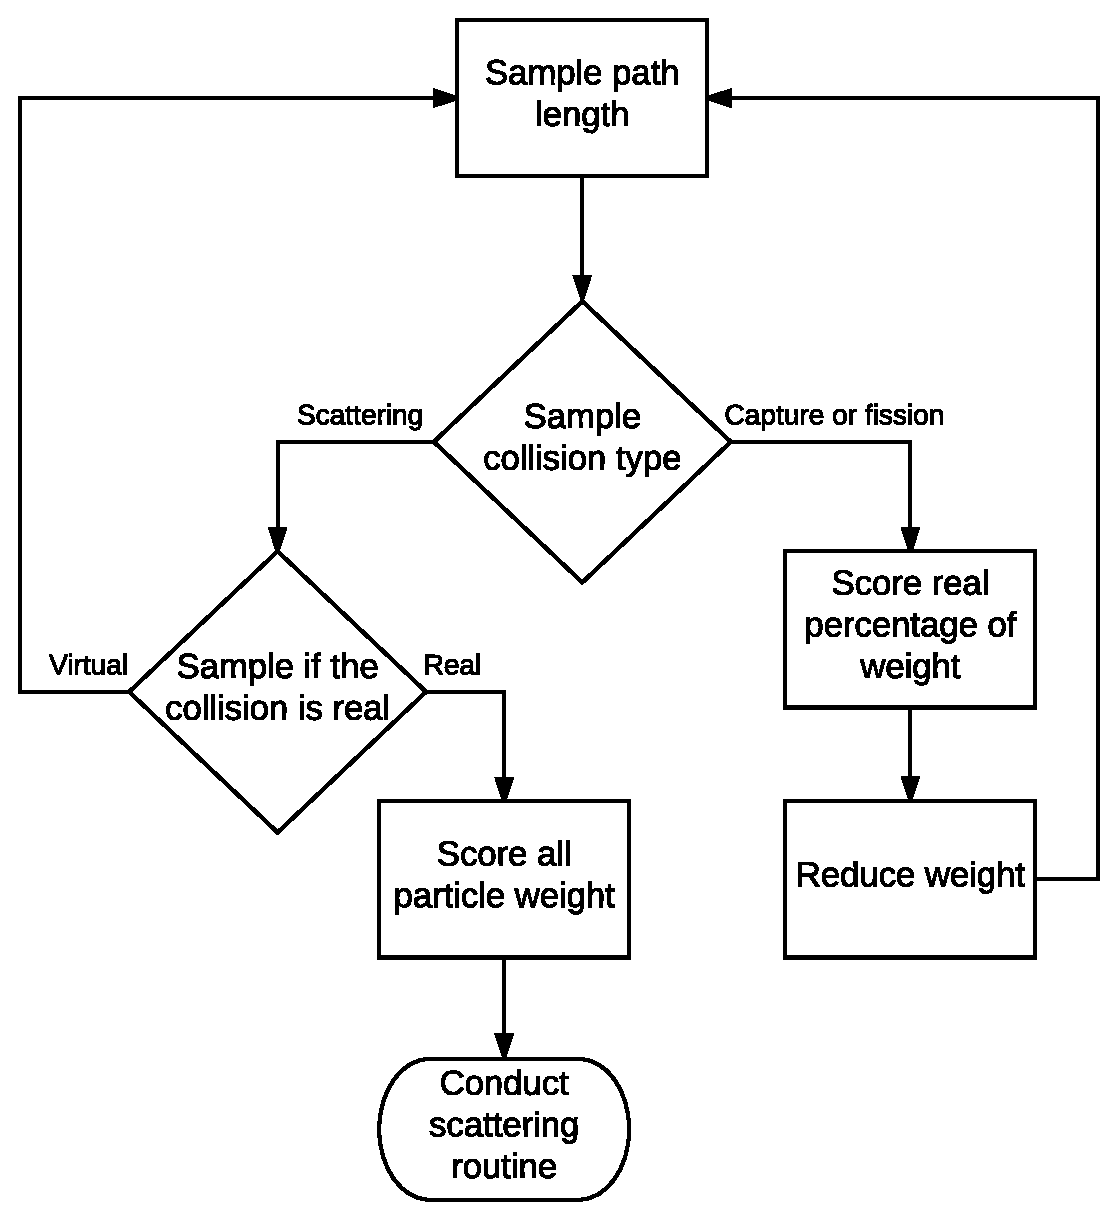
\includegraphics[scale=0.5]{images/wdt}
  \caption{\Acrlong{wdt} with scattering rejection sampling.\label{fig:wdt}}
\end{figure}
Note that there are two separate scoring events in each collision
subroutine: scoring of the actual collision type for calculating
specific reaction rates, and scoring of collision itself used by the
collision flux estimator. In addition, scoring the fission reaction
also encompasses generation of fission neutrons.

In the original delta-tracking routine, the rejection sampling takes
place prior to collision type sampling, and collision scoring can
occur between the two. This is the routine that Serpent 2 used, prior
to modification for the above scheme. By moving the rejection sampling
after the collision type sampling, the collision score is no longer
agnostic of the type of collision that will occur. Therefore, in the
implementation of this routine in Serpent 2, the collision scoring was
moved after the collision type sampling.

\section{Implementation in Serpent 2}
\label{sec:method_implementation}

The \gls{wdt} algorithm is implemented to work alongside the current
implementation of ray tracing and delta-tracking, as described in
Sec.~\ref{sec:serpent2}. \gls{wdt} is designed to improve the
effectiveness of delta-tracking when the change of a virtual collision
is high. We can hypothesize that the algorithm will benefit in the
regime where $P_{\mathrm{real}}$ is low. At high values of
$P_{\mathrm{real}}$, a majority of the weight of the incoming particle
is scored. This leaves the particle that undergoes a virtual collision
with a very low weight, relying on the rouletting routine to prevent
causing computational inefficiency. These two situations imply that
there is a region between low and high values of $P_\mathrm{real}$
where \gls{wdt} may provide benefit.

A new input parameter line \verb|set wdt| is used to indicate that
\gls{wdt} is to be used, and can also set the value of the \gls{wdt}
threshold $t_{\mathrm{wdt}}$. This is the ratio below which \gls{wdt} will be used. This
scheme is summarized in Fig.~\ref{fig:ray_wdt}.
\begin{figure}[hbtp]
  \centering
  \begin{align*}
    \mathrm{Mode} =
    \begin{cases}
      \mathrm{Ray tracing}, & P_\mathrm{real} < 1-c \\
      \mathrm{\gls{wdt}}, & 1-c \leq P_\mathrm{real} < t_{\mathrm{wdt}}
      \\
      \mathrm{Delta-tracking}, & P_\mathrm{real} \geq t_{\mathrm{wdt}}
    \end{cases}
  \end{align*}
  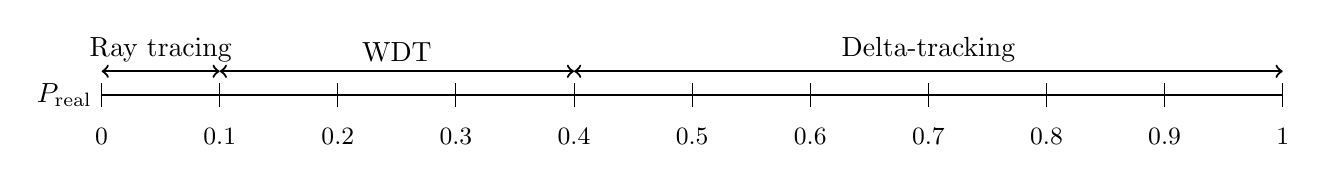
\begin{tikzpicture}[scale=1.5]
    \draw[thick] (0,0) -- (10.0,0);
    \foreach \x in {0,1,...,10}
    {
      \draw (\x, 0.1) -- (\x, -0.1);
      \pgfmathsetmacro\result{\x * 0.1}
      \node [below] at (\x, -0.2) {\small $\pgfmathprintnumber{\result}$};
    }
    \node [left] at (0,0) {$P_{\mathrm{real}}$};
    \draw[ thick, <->] (0,0.2) -- (1,0.2);
    \draw[ thick, <->] (1,0.2) -- (4,0.2);
    \draw[ thick, <->] (4,0.2) -- (10,0.2);
    \node [above] at (0.5, 0.2) {Ray tracing};
    \node [above] at (2.5, 0.2) {WDT};
    \node [above] at (7, 0.2) {Delta-tracking};
  \end{tikzpicture}
  \caption[Implemented selection scheme for ray-tracing, weighted and normal
    delta-tracking.]{Implemented selection scheme for ray-tracing, weighted and normal
    delta-tracking. Shown using the values of $(1-c)=0.1$ and $t_{\mathrm{wdt}}=0.4$.}
  \label{fig:ray_wdt}
\end{figure}



%%% Local Variables:
%%% mode: latex
%%% TeX-master: "../masters_report"
%%% End:
